\chapter{Iteración I - Agente HTN}
\label{chap:iter1}

\lettrine{E}{n} esta primera iteración, se aborda la planificación simbólica
usando un planificador jerárquico de tareas (\gls{htn}), que sirve de base
para la comparación con el resto de algoritmos gracias a su carácter determinista 
y explicable.

Como resultado de esta iteración se obtienen dos elementos: un agente
que actúa como \textit{baseline} frente a las técnicas de
aprendizaje, y un \textit{dataset} propio de demostraciones generado a partir de
sus ejecuciones para entrenar en el Capítulo~\ref{chap:iter2}.

\section{Diseño}
La tarea objetivo \gls{woodcutting} consiste en la recolección de $k$ troncos de un tipo específico de madera.
Esta tarea objetivo se descompone en una tarea compuesta que se
resuelve aplicando repetidamente una secuencia de primitivas (Figura~\ref{fig:htn-tree}, página~\pageref{fig:htn-tree}).

\begin{figure}[htbp]
  \centering
  \begin{forest}
    for tree={
      font=\footnotesize, grow'=0, folder, rounded corners, draw,
      edge={-, semithick}, l sep=4mm, s sep=1.2mm, anchor=west,
      inner sep=2.5pt,
    },
    compuesta/.style={fill=blue!8},
    primitiva/.style={fill=green!12},
    recup/.style={fill=red!10},
    [{Recolectar $k$ troncos \textit{(post-cond.: hasItem)}}, compuesta
      [{Obtener tipo de madera \textit{(obtainWoodType)}}, primitiva]
      [{Talar tronco --- repetir hasta $k$}, compuesta
        [{Buscar árbol visible en cono \gls{fov} \textit{(findNearestVisibleBlock)}}, primitiva]
        [{Explorar si no hay árbol \textit{(exploreRandom)}}, recup]
        [{Ir al árbol \textit{(moveToBlock)}}, primitiva]
        [{Talar el tronco completo \textit{(mine)}}, compuesta
          [{Talar y recoger el bloque base \textit{(collectBlock)}}, primitiva]
          [{Moverse y talar el resto \textit{(mineTreeTrunk)}}, primitiva]
        ]
      ]
    ]
  \end{forest}
  \caption[Árbol de descomposición de la tarea de woodcutting]{Árbol de
  descomposición \gls{htn} de la tarea de \gls{woodcutting}. La tarea compuesta
  se descompone en una primitiva de selección de madera y en una
  tarea compuesta de tala que se repite hasta conseguir los $k$ troncos. Las tareas
  \textbf{compuestas} se muestran en \textbf{azul}, las \textbf{primitivas} en \textbf{verde} 
  y la \textbf{recuperación} en \textbf{rojo}.}
  \label{fig:htn-tree}
\end{figure}

Cada tarea se define mediante: una \textbf{pre-condición}, estado del mundo antes de la ejecución;
una \textbf{post-condición}, estado del mundo después de la ejecución; y un \textbf{método}, forma de resolver la tarea usando 
una secuencia de subtareas (primitivas u otras compuestas). 
Estas restricciones son las que otorgan al agente su carácter \textbf{determinista} (ante el
mismo estado toma siempre la misma decisión) e \textbf{interpretable} (cada acción
corresponde a una regla).

La condición de éxito de la tarea de \gls{woodcutting} es tener $k$ troncos en
el inventario. Al ser una tarea objetivo, no se ejecuta de forma directa, sino que se
descompone en la tarea compuesta de talar un árbol, que se repite hasta alcanzar
los $k$ troncos. Talar un árbol implica, a su vez, varios pasos: localizar un tronco
dentro del \gls{fov} (y, si no hay ninguno, explorar el mundo hasta que aparezca
uno), desplazarse hasta él y, finalmente, talar el tronco completo. Cada uno de estos
pasos se descompone de nuevo hasta llegar a primitivas como mover la cámara o minar un bloque.

Al ser una de las primeras tareas a realizar en \textit{Minecraft}, la tarea \gls{woodcutting} no presenta realmente pre-condiciones, ya que el agente puede empezar a talar en cualquier momento. Sin embargo, en tareas posteriores como la obtención de un pico de hierro es necesario que el agente tenga las herramientas adecuadas (véase el Apéndice~\ref{apx:htn-iron-decomp}).

\section{Tareas Primitivas}
Las tareas primitivas que componen la tarea de \gls{woodcutting} se recogen
en la Tabla~\ref{tab:htn-primitivas} (página~\pageref{tab:htn-primitivas}). Cada primitiva se traduce en una acción
básica realizable en \textit{Minecraft} (moverse, minar, mover la cámara\dots) y 
se apoya en la \acrshort{api} de \textit{Mineflayer} descrita en el Capítulo~\ref{chap:arquitectura}.

\begin{table}[htbp]
  \centering
  \resizebox{\textwidth}{!}{%
  \small
  \rowcolors{2}{white}{udcgray!25}
  \begin{tabular}{c|c}
  \rowcolor{udcpink!25}
  \textbf{Primitiva} & \textbf{Función} \\\hline
  \textit{obtainWoodType}          & Determinar el tipo de madera  \\
  \textit{findNearestVisibleBlock} & Localizar el tronco visible más cercano (\gls{fov}) \\
  \textit{moveToBlock}             & Navegar al bloque mediante un \gls{pathfinder} \\
  \textit{collectBlock}            & Obtener un bloque y recogerlo \\
  \textit{mineTreeTrunk}           & Talar una secuencia de bloques \\
  \textit{exploreRandom}           & Explorar si no hay árbol visible (recuperación) \\
  \end{tabular}
  }
  \caption[Primitivas del agente simbólico para la tarea de woodcutting]{Primitivas del agente simbólico para la tarea de \textit{woodcutting}.}
  \label{tab:htn-primitivas}
\end{table}

\paragraph{Selección del tipo de madera:}
utilizando la \acrshort{api} de \textit{Mineflayer}
se identifica el \gls{bioma} y, mediante un mapeo predefinido, se determina el tipo de madera objetivo a talar
(por ejemplo, \textit{forest} $\rightarrow$ \textit{oak\_log}); si el bioma no está mapeado, se recurre a una
búsqueda visual de los tipos de tronco más comunes en el entorno. Si no hay
madera visible al alcance, la tarea falla en lugar de consultar la posición
omnisciente de los bloques, en coherencia con la restricción de percepción del
Capítulo~\ref{chap:arquitectura}. 

\paragraph{Búsqueda de Bloques en el Cono de Visión:}
la localización de troncos reutiliza el mismo mecanismo de percepción definido en
el Capítulo~\ref{chap:arquitectura}. La búsqueda se restringe al 
\gls{fov} del agente y exige línea de visión directa, de modo que el agente solo
considera los árboles que un jugador humano vería. La primitiva de
talar usa esta búsqueda para evitar información del mundo fuera del \gls{fov}.

\paragraph{Tala del Tronco:}
una vez localizado el bloque, la tala no vuelve a invocar
la búsqueda por \gls{fov} para los bloques superiores. En su lugar,
\textit{mineTreeTrunk} recorre verticalmente la posición
ya conocida: mina el bloque en $(x,\,y{+}1,\,z)$, comprueba si el bloque
en $(x,\,y{+}n,\,z)$ es del mismo tipo de tronco, y así sucesivamente hasta
que el tipo de bloque cambia. Esta estrategia permite talar un árbol completo
sin necesidad de reposicionarse ni relanzar el \gls{pathfinder} para cada bloque.

\paragraph{Exploración de Recuperación:}
cuando la búsqueda en el \gls{fov} no encuentra ningún árbol,
el agente no puede determinar si existe madera en el mundo o si simplemente no
es visible desde su posición actual. En este caso se activa \textit{exploreRandom},
que elige una dirección aleatoria y pide al \gls{pathfinder} avanzar hasta \num{30} bloques
en esa dirección, permaneciendo en la superficie
para evitar posiciones subterráneas donde no se encuentra madera. Durante la exploración, se
comprueba cada \qty{500}{ms} si ha aparecido algún tronco en el \gls{fov}; si es así, la
exploración se interrumpe y se retoma la tala.

\paragraph{Progresión y Recuperación de Fallos:}
la ejecución de cada tarea contiene una 
lógica de recuperación (Figura~\ref{fig:htn-recovery}, página~\pageref{fig:htn-recovery}). 
Antes de actuar se comprueba la post-condición;
mientras no se cumpla, se ejecuta el método de la tarea hasta un máximo de $N$
intentos. Si un intento lanza un error (por ejemplo, el objetivo ha desaparecido), 
se dispara un mecanismo de recuperación: una acción de recuperación
específica de la tarea o, si no existe, una exploración aleatoria del entorno
para reposicionar al agente antes de reintentar. 
Si el agente se queda sin intentos, la tarea se aborta y se propaga el fallo a la tarea padre,
o bien, se detiene la ejecución si es la tarea raíz, marcando la ejecución como fallida.

\begin{figure}[htbp]
  \centering
  \resizebox{\textwidth}{!}{%
  \begin{tikzpicture}[
    font=\footnotesize, >=Latex,
    proc/.style ={draw, rounded corners, align=center, minimum width=26mm, minimum height=8mm, fill=ficblue!8},
    dec/.style  ={draw, diamond, aspect=2.4, align=center, inner sep=1pt, fill=udcgray!8},
    term/.style ={draw, rounded corners, align=center, minimum width=24mm, minimum height=8mm},
  ]
    \node[dec] (post) {¿Post-cond.?};
    \node[proc] (met) [right=12mm of post] {Ejecutar método};
    \node[dec]  (int) [right=12mm of met] {¿Quedan intentos?\\{\scriptsize(máx.\ $N$)}};
    
    \node[term, fill=udcpink!25]  (abort) [right=12mm of int] {ABORTAR};
    \node[term, fill=green!12] (comp) [above=12mm of post] {COMPLETADO};
    \node[term, fill=udcgray!8] (padre) [below=10mm of abort] {Tarea padre};
    
    \node[proc, fill=udcpink!8] (rec)   [below=12mm of int]  {Recuperación\\{\scriptsize exploración, atascos}};

    \draw[->] (post) -- node[left]{sí} (comp);
    \draw[->] (post) -- node[above]{no} (met);
    \draw[->] (met)  -- node[above]{error} (int);
    \draw[->] (int)  -- node[above]{no} (abort);
    \draw[->] (int)  -- node[right]{sí} (rec);
    \draw[->] (abort) -- (padre);

    \path (rec.south) -- ++(0,-6mm) coordinate (ret_y);
    
    \draw[-] (rec.south) |- (met.south |- ret_y);
    \draw[->] (met.south) -- node[right]{éxito} (met.south |- ret_y);
    \draw[->] (met.south |- ret_y) -| (post.south);
    
  \end{tikzpicture}
  }
  \caption[Bucle de ejecución de una tarea]{Bucle de ejecución de una tarea
  (\textit{runSmartTask}) del \gls{htn}. Antes de cada intento se comprueba la post-condición; mientras no
  se cumpla, se ejecuta el método de la tarea. Si un intento falla, se dispara un mecanismo de
  recuperación (una acción específica o una exploración aleatoria) y se reintenta, hasta un
  máximo de $N$ intentos. Si se agotan, la tarea se aborta y propaga el fallo a la tarea padre.}
  \label{fig:htn-recovery}
\end{figure}


Se añaden dos prevenciones extra debido a las limitaciones de la simulación. La primera consiste en una comprobación periódica de
la posición del agente mientras el \gls{pathfinder} está activo; si no avanza lo suficiente durante varias
muestras consecutivas (por ejemplo, si el agente se queda atascado), se reinicia la navegación. 
La segunda es un \textit{timeout} global por episodio que limita la
duración máxima de una ejecución para evitar bucles infinitos.

\section{Generación del Dataset de Demostraciones}
\label{sec:dataset-htn}
Al comenzar la implementación del agente de imitación (Capítulo~\ref{chap:iter2})
surgió la necesidad de un conjunto de demostraciones de un experto. Una de las opciones
sería reutilizar un \textit{dataset} público como \textit{MineRL}~\cite{guss2019minerl},
cuyo subdataset \textit{Treechop-v0} aborda precisamente la misma tarea. Sin
embargo, su uso resulta imposible en este trabajo por los motivos mencionados en el 
Capítulo~\ref{chap:metodologia}.

Por todo ello, en lugar de adaptar un \textit{dataset} ajeno se genera uno propio
ejecutando el agente \gls{htn} sobre el mismo entorno en el que se evalúan las técnicas.
Al compartir exactamente el mismo entorno, espacio de acciones y espacio de observación
que el agente de imitación, las demostraciones no necesitan ninguna conversión y
sus etiquetas coinciden con el conjunto de acciones del modelo. Esto
garantiza la coherencia entre el experto y el aprendiz y elimina el desajuste de
formato y granularidad de \textit{datasets} externos.

Durante la ejecución se almacenan pares
\textit{OBSERVACIÓN-ACCIÓN} que conformarán el \textit{dataset}. A intervalos regulares se captura un \textit{frame} 
que combina la imagen del visor en primera persona (véase el Apéndice~\ref{apx:frame}), el vector de estado del agente
de la Tabla~\ref{tab:obs-space} (página~\pageref{tab:obs-space}) y la acción que está ejecutando en ese
instante. Cabe destacar que no se incluyen los movimientos de la cámara como acciones discretas, ya que el agente 
los realiza sobre posiciones absolutas del mundo; es decir, no emplea acciones como \textit{camera\_right}, 
sino que orienta su visión directamente mediante funciones como \textit{lookAt(x,y,z)}.
Los \textit{frames} sin acción se descartan (por ejemplo, los capturados durante el tiempo de inicialización, 
donde el agente aún no interactúa con el entorno).
La estructura final de estos \textit{frames} se detalla en la Tabla~\ref{tab:dataset-frame} (página~\pageref{tab:dataset-frame}).

\begin{table}[htbp]
  \centering
  \resizebox{\textwidth}{!}{%
  \small
  \rowcolors{2}{white}{udcgray!25}
  \begin{tabular}{c|c|c}
  \rowcolor{udcpink!25}
  \textbf{Campo} & \textbf{Tipo / Rango} & \textbf{Descripción} \\\hline
  \textit{image}                & PNG               & Vista en primera persona del visor \\
  \textit{x, y, z}              & float (bloques)   & Posición del agente \\
  \textit{yaw, pitch}           & float (rad)       & Orientación de la cámara \\
  \textit{action}               & categórica        & Acción discreta ejecutada en el \textit{frame} \\
  \textit{dyaw, dpitch}         & float (rad)       & Desplazamiento de cámara respecto al \textit{frame} anterior \\
  \textit{tree\_visible}        & $\{0, 1\}$        & Árbol dentro del \gls{fov} \\
  \textit{tree\_distance}       & float (bloques)   & Distancia al árbol visible más cercano \\
  \end{tabular}
  }
  \caption[Estructura de los \textit{frames} del dataset.]{Estructura de los \textit{frames} del \textit{dataset} de demostraciones
  generado por el \gls{htn}. La posición absoluta se guarda para calcular el desplazamiento entre \textit{frames} posteriormente.}
  \label{tab:dataset-frame}
\end{table} 

La distribución de acciones del \textit{dataset}, ilustrada en la Figura~\ref{fig:dataset-clases} (página~\pageref{fig:dataset-clases}), está desbalanceada.
Esto se debe a que el agente simbólico dispone de información completa del entorno a través de la \acrshort{api},
lo que le permite actuar de forma muy eficiente. Por ejemplo, conoce la posición exacta de los árboles y, 
mediante el uso del \gls{pathfinder}, calcula rutas óptimas que rara vez incluyen movimientos laterales o hacia atrás. 
Como consecuencia, aunque el espacio de acciones contiene acciones como saltar, moverse a la derecha o moverse a la izquierda, 
el agente solo ejecuta las más eficientes para completar la tarea. Este comportamiento provoca que ciertas 
acciones aparezcan con muy poca frecuencia en el \textit{dataset}, lo que motiva el descarte de las clases menos representadas.

\begin{figure}[htbp]
  \centering
  \resizebox{\textwidth}{!}{%
  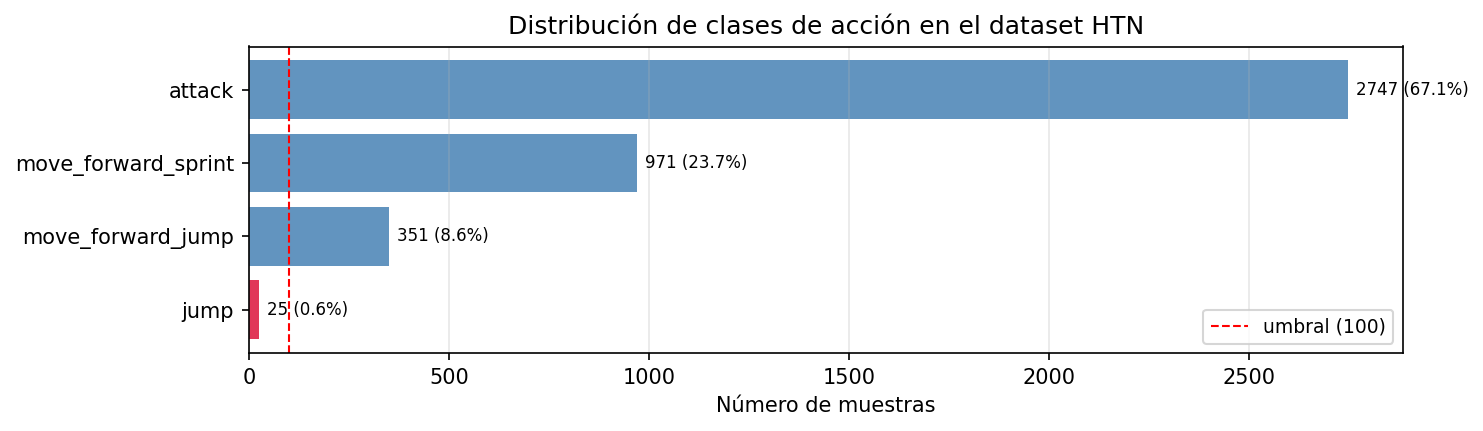
\includegraphics[width=1\textwidth]{imaxes/06_htn/dataset_clases.png}
  }
  \caption[Distribución de clases de acción en el dataset HTN]{Distribución de
  las clases de acción en el \textit{dataset} de demostraciones generado por el agente
  simbólico tras \num{118} ejecuciones.}
  \label{fig:dataset-clases}
\end{figure}

El registro de la acción discreta y la variación de la cámara es lo que
permite entrenar una arquitectura de doble cabeza (clasificación de la acción y 
regresión del movimiento de cámara correspondiente a la acción) en el Capítulo~\ref{chap:iter2}. Tras una
limpieza que descarta episodios con errores y acciones poco
representativas, el \textit{dataset} resultante consta de los episodios y \textit{steps}
detallados en la Tabla~\ref{tab:datasets} (página~\pageref{tab:datasets}).

\section{Resultados de la Iteración}
El agente simbólico se evalúa sobre la misma tarea de entrenamiento, \gls{woodcutting}, ejecutando un
conjunto de episodios con reinicio determinista (Capítulo~\ref{chap:arquitectura}).
Cada episodio registra: los troncos recogidos, los troncos rotos y la duración; la tasa de éxito se calcula con la
métrica común de todas las técnicas (recoger al menos $k$ troncos, con $k=5$), lo que garantiza una comparación justa en el
Capítulo~\ref{chap:discusion-resultados}.

Sobre un total de \num{50} episodios, el agente alcanza una tasa de éxito del \qty{100.0}{\percent}. La
distribución por episodio de troncos, tiempo y pasos se resume en la
Tabla~\ref{tab:htn-eval} (página~\pageref{tab:htn-eval}).

\begin{table}[htbp]
  \centering
  \rowcolors{3}{white}{udcgray!25}
  \resizebox{\linewidth}{!}{
      \begin{tabular}{ccc|ccc|ccc}
      \rowcolor{udcpink!25}
       & & & \multicolumn{3}{c|}{\textbf{Troncos}} & \multicolumn{3}{c}{\textbf{Tiempo (s)}} \\
      \rowcolor{udcpink!25}
      \textbf{Técnica} & \textbf{Eps.} & \textbf{Éxito (\%)} & \textbf{$\mu$} & \textbf{$\tilde{x}$} & \textbf{$\sigma$} & \textbf{$\mu$} & \textbf{$\tilde{x}$} & \textbf{$\sigma$} \\\hline
      HTN & \num{50} & \num{100.0} & \num{6.00} & \num{6.00} & \num{0.00} & \num{26.7} & \num{26.4} & \num{1.1} \\
      \end{tabular}
  }
  \caption[Evaluación de la técnica simbólica]{Evaluación de la técnica \gls{htn} bajo la métrica común recoger $k=5$ troncos. Troncos y tiempo por episodio: 
  media ($\mu$), mediana ($\tilde{x}$), y desviación típica ($\sigma$).}
  \label{tab:htn-eval}
\end{table}

Como \textit{baseline}, el agente simbólico ofrece un comportamiento robusto e
interpretable sin necesidad de entrenamiento. La limitación principal
es la dependencia del conocimiento del dominio definido
manualmente: el rendimiento está condicionado por la calidad de las primitivas y
de la navegación, y los fallos pueden provenir sobre todo de situaciones de atasco o de
escenarios en los que no hay madera visible al alcance. 
La tarea empleada para la evaluación es una de las más simples de \textit{Minecraft}, precedida solo
por la de \gls{navegacion}. Las siguientes tareas a realizar según el
árbol de progresión del juego (véase el Apéndice~\ref{apx:htn-iron-decomp})
presentan un incremento significativo de complejidad, al requerir un mayor número de subtareas
y dependencias entre recursos.

Para la realización de las tareas el agente \gls{htn} utiliza información que no es común para el 
jugador (posiciones exactas, visión y movimiento perfectos\dots); aunque sí obtenible, manteniendo la
restricción de omnisciencia. Esto plantea la necesidad de recurrir al \gls{aprendizaje-automatico}, 
utilizando la misma información que usaría un jugador real. 
Si bien la obtención de los datos para el enfoque automático puede ser una tarea ardua, 
su horizonte puede resultar menos limitado que el del enfoque simbólico.

\section{Escalabilidad a tareas de horizonte largo}
La \gls{htn} no se limita a la tala de madera. La misma arquitectura de tareas
compuestas, primitivas y recuperación escala a la progresión completa hasta el pico
de hierro (véase el Apéndice~\ref{apx:htn-iron-decomp}), que encadena
tres fases: madera, piedra y hierro. 

\subsection{Dependencias entre tareas: precondiciones}
En el \gls{woodcutting} la única dependencia real es conocer el tipo de madera del
\gls{bioma}. En cambio, la progresión hasta el hierro encadena requisitos estrictos:
no se puede minar piedra sin un pico de madera, ni hierro sin un pico de piedra,
ni fundir sin un horno.

El planificador gestiona esto mediante precondiciones recursivas: antes de ejecutar
una tarea comprueba si se cumple el estado que necesita y, si no, lo resuelve como
subtarea. Por ejemplo, minar piedra exige un pico de madera
(\textit{ensureEquipped}); si el agente no lo tiene, lo fabrica, lo que a su vez
requiere tablones y una mesa de trabajo (\textit{ensureWoodAndPlanks},
\textit{ensureCraftingTable}).

La Figura~\ref{fig:htn-precond} (página~\pageref{fig:htn-precond}) ilustra ese descenso recursivo.

\begin{figure}[htbp]
  \centering
  \resizebox{\textwidth}{!}{%
  \begin{tikzpicture}[
    font=\footnotesize, >=Latex,
    every node/.style={align=center},
    % Usamos text width para forzar saltos de línea y estrechar los nodos
    goal/.style ={draw, rounded corners, fill=blue!20,  text width=20mm, inner sep=4pt},
    proc/.style ={draw, rounded corners, fill=udcgray!8,  text width=28mm, inner sep=4pt},
    leaf/.style ={draw, rounded corners, fill=green!12,   text width=22mm, inner sep=4pt},
    recup/.style={draw, rounded corners, fill=udcpink!8,  text width=26mm, inner sep=4pt},
    edgelbl/.style={font=\scriptsize\itshape, align=center, inner sep=2pt},
  ]
    
    % Eje principal (Horizontal)
    \node[goal] (mine)  {Minar\\piedra};
    \node[proc] (equip) [right=10mm of mine]  {\textit{ensureEquipped}\\(pico madera)};
    \node[proc] (craft) [right=10mm of equip] {\textit{craftItem}\\(pico madera)};

    % Rama 1: Madera (Hacia arriba y a la derecha)
    \node[proc]  (wood)   [above right=10mm and 12mm of craft] {\textit{ensureWoodAndPlanks}};
    \node[recup] (chop)   [right=10mm of wood]  {\textit{chop}\\(si faltan troncos)};
    \node[leaf]  (planks) [right=8mm of chop]  {\textit{craftItem}\\(tablones)};

    % Rama 2: Mesa de trabajo (Hacia abajo y a la derecha)
    \node[proc] (table)  [below right=10mm and 12mm of craft] {\textit{ensureCraftingTable}};
    \node[leaf] (mktab)  [right=12mm of table] {\textit{craftItem}\\(mesa)};
    \node[leaf] (place)  [right=12mm of mktab] {\textit{placeBlock}\\(colocar)};

    % Conexiones eje principal
    \draw[->] (mine)  -- node[edgelbl,above]{requiere} (equip);
    \draw[->] (equip) -- node[edgelbl,above,text width=14mm]{si falta,\\fabrica} (craft);
    
    % Conexiones bifurcadas (salen de las esquinas para no cruzarse)
    \draw[->] (craft.north east) -- node[edgelbl,above left,pos=0.5]{requiere} (wood.south west);
    \draw[->] (craft.south east) -- node[edgelbl,below left,pos=0.5]{requiere} (table.north west);
    
    % Conexiones rama 1
    \draw[->] (wood)  -- node[edgelbl,above]{si falta} (chop);
    \draw[->] (chop)  -- (planks);
    
    % Conexiones rama 2
    \draw[->] (table) -- node[edgelbl,above]{si falta} (mktab);
    \draw[->] (mktab) -- (place);
    
  \end{tikzpicture}
  }
  \caption[Resolución recursiva de precondiciones]{Resolución recursiva de
  precondiciones para minar piedra. Cada tarea garantiza el estado que necesita
  antes de aplicarse: si una precondición no se cumple, se resuelve como subtarea
  (en \textbf{azul} la tarea objetivo, en \textbf{gris} las tareas compuestas,
  en \textbf{verde} las primitivas y en \textbf{rosa} la recuperación). El descenso
  encadena la obtención de madera, la fabricación de tablones y la colocación de la
  mesa de trabajo, hasta poder fabricar el pico de madera.}
  \label{fig:htn-precond}
\end{figure}

\subsection{Alcance del planificador}
El planificador ejecuta la jerarquía de forma determinista: descompone el objetivo en
las fases necesarias, resuelve las precondiciones y realiza las acciones sin
entrenamiento. Las fases de madera y piedra se ejecutan con fluidez porque los
recursos están en la superficie y dentro del \gls{fov}. La fase de hierro introduce
una dificultad adicional: el mineral se genera en torno a $Y=15$-$16$ sin una
posición $(X,Z)$ conocida de antemano, por lo que localizarlo requiere una
exploración subterránea a ciegas que alarga los episodios y los hace poco
reproducibles. Por ese motivo en este trabajo no se presenta una métrica de la
progresión completa, sino únicamente de la tarea de \gls{woodcutting}.